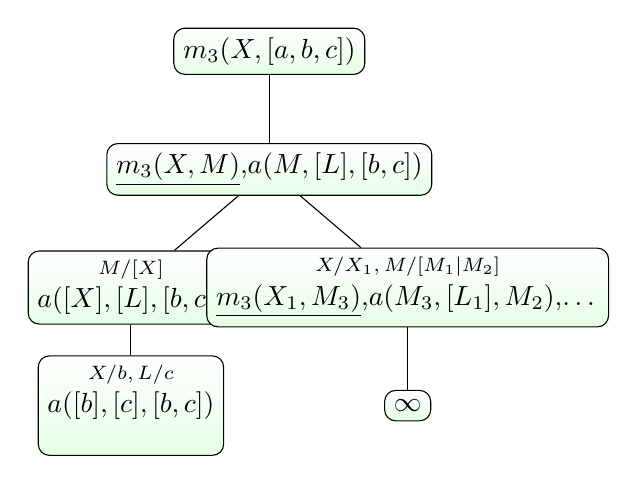
\begin{tikzpicture}[sibling distance=10em,
    every node/.style = {shape=rectangle, rounded corners,
      draw, align=center,
      top color=white, bottom color=green!10}]]
    \node {$m_3(X,[a,b,c])$}
      child { node {\underline{$m_3(X, M)$},$a(M, [L], [b,c])$}
        child { node {\scriptsize $M/[X]$\\$a([X], [L], [b,c])$}
          child { node {\scriptsize $X/b, L/c$\\$a([b],[c],[b,c])$\\$\blacksquare$}}
        }
        child {node {\scriptsize $X/X_1, M/[M_1|M_2]$\\\underline{$m_3(X_1,M_3)$},$a(M_3,[L_1],M_2)$,\ldots}
          child {node {$\infty$}}
        }
      };
  \end{tikzpicture}